\documentclass[a4paper, 12pt]{article}%тип документа

%отступы
\usepackage[left=1.5cm,right=1cm,top=2cm,bottom=3cm,bindingoffset=0cm]{geometry}
\setlength{\parindent}{5ex}
%Русский язык
\usepackage[T2A]{fontenc} %кодировка
\usepackage[utf8]{inputenc} %кодировка исходного кода
\usepackage[english,russian]{babel} %локализация и переносы

%Вставка картинок
\usepackage{graphicx}
\graphicspath{{pictures/}}
\DeclareGraphicsExtensions{.pdf,.png,.jpg,}
\usepackage{wrapfig}

%Графики
\usepackage{pgfplots}
\pgfplotsset{compat=1.9}

%Математика
\usepackage{amsmath, amsfonts, amssymb, amsthm, mathtools}

%Таблицы
\usepackage{longtable} 
\usepackage{float}

%Римские цифры
\newcommand{\RomanNumeralCaps}[1]{\uppercase\expandafter{\romannumeral#1}}

\usepackage{multirow}



\begin{document}
	\begin{titlepage}
		\begin{center}
			\textsc{Федеральное государственное автономное образовательное учреждение высшего образования«Московский физико-технический институт (национальный исследовательский университет)»\\[5mm]
			}
			
			\vfill
			
			\textbf{Отчёт по лабораторной работы 4.3.6\\[3mm]
				Саморепродукция
				\\[50mm]
			}
			
		\end{center}
		
		\hfill
		\begin{minipage}{.5\textwidth}
			Выполнил студент:\\[2mm]
			Сериков Василий Романович\\[2mm]
			группа: Б03-102\\[5mm]
			
		\end{minipage}
		\vfill
		\begin{center}
			Москва, 2023 г.
		\end{center}
		
	\end{titlepage}
	
	\newpage
	\setcounter{page}{2}
	\textbf{Аннотация}\\
	
	\textbf{Цель работы: }\\
	
	Изучение явления саморепродукции и применение его к измерению параметров периодических структур.\\
	
	\textbf{В работе используются: } \\
	
	Лазер, кассета с сетками, мира, короткофокусная линза с микрометрическим винтом, экран, линейка.\\
	
	\textbf{Теория: }\\
	
	При дифракции на предмете с периодической структурой наблюдается явление саморепродукции: на некотором расстоянии от предмета вдоль направления распространения волны появляется изображение, которое потом периодически повторяется.  \par
	
	Найдём выражение для расстояния между этими плоскостями. Плоской монохроматической волной называется волна вида
	$$
	E(r, t)=a_0 e^{-\gamma\left(\omega t-k r-\psi_0\right)}
	$$
	где амплитуда $\Omega_0-$ действительная постоянная, $\omega$ - круговая частота, $k$ - волновой вектор $(|k|=2 \pi / \lambda), \psi_0-$ начальная фаза. Колебания происходят синфазно во всех точках плоскости:
	$$
	k r=u x+v y+\sqrt{k^2-u^2-v^2}, z=\text { const. }
	$$
	
	Направление распространения плоской монохроматической волны характеризуется волновым вектором $k$, а $u$ и $v$ есть проекции его на оси координат $x$ и $y$ соответственно. В дальнейшем мы будем опускать зависимость от времени $e^{-i \omega t}$ и использовать для описания монохроматической волны комплексного амплитуду. Для плоской волны (1) комплексную амплитуду можно представить в виде
	$$
	\begin{array}{l} 
		f(x, y, z)=a_0 e^{i \psi_0} e^{i(u x+v y)} e^{i \sqrt{k^2-u^2-v^2}, z} \\
		\quad=f(x, y, 0) \cdot e^{i \sqrt{k^2-u^2-v^2} \cdot y} .
	\end{array}
	$$
	Таким образом, для того чтобы получить комплексную амплитуду плоской волны в произвольной плоскости $z=$ const, надо ее значение в плоскости $z=0$ домножить на фазовый множитель $e^{i \sqrt{k^2-u^2-v^2}, z}$.
	
	Представим волну за периодическим объектом в виде суммы плоских волн разных направлений. Отдельные слагаемые плоские волны называют пространственными гармониками. Вдоль пути распространения волнового фронта на некотором расстоянии $z_0$ от предмета существует плоскость, где разность фазовых набегов любых пространственных гармоник (плоских волн идущих под углом $\theta$т к оси распространения), входящих в состав суперпозиции, кратна $2T$ В этой плоскости фазовые соотношения между всеми плоскими волнами, входящими в состав суперпозиции, такие же, что и в предметной плоскости. Поэтому в результате интерференции этих волн возникает изображение, тождественное исходному периодическому объекту. Все сказанное справедливо для любого расстояния $z_n$, кратного $z_0$. Для решетки с периодом $d$.
	\begin{equation}
		z_n = \frac{2d^2}{\lambda}n
	\end{equation}
	
	Суть эксперимента по саморепродукции состоит в том, что дифрагированная на периодическом транспаранте (решетка, сетка) плоская монохроматическая волна лазера (лазерный пучок) воспроизводит изображение транспаранта без каких-либо оптических элементов.
	
	\begin{figure}[H]
		\centering
		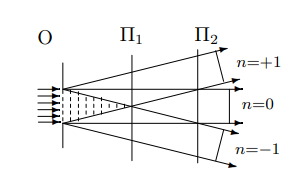
\includegraphics[scale=2]{fig1.png}
		\caption{Принципиальная схема
			дифракции на сетке. Между сеткой 0 и плоскостью
			П1 наблюдаются репродуцированные изображения сетки}
	\end{figure}

	\begin{figure}[H]
	\centering
	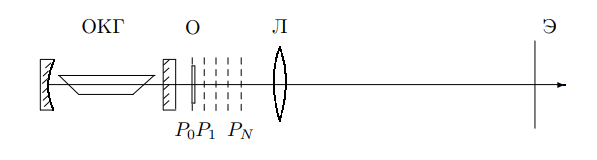
\includegraphics[scale=1.5]{ust.png}
	\caption{Схема установки: ОКГ
		— гелий-неоновый лазер, 0 — двумерная решетка,
		PN
		— плоскости, где наблюдаютс
		я репродуцированные
		изображения,
		Л
		—
		короткофокусная линза,
		Э
		— экран для наблюдения изображения объекта}
	\end{figure}
	
	
	\newpage
	
	\textbf{Ход работы: }\\
	
	\begin{enumerate}
		
		
		
		\item Определим период решёток по их пространственному спектру. Для каждой сетки определим расстояние x между соседними дифракционными максимумами на экране: измерим расстояние X между двумя достаточно удалёнными друг от друга максимумами и поделим на число промежутков m между ними (x = X/m = f(№)).
		
		По результатам измерений спектра получим период каждой решётки по формуле $ d = L\frac{\lambda}{x}, \lambda = 532$ нм. Полученные результаты занесем в таблицу 1.
		
		\begin{longtable}{|c|c|c|c|c|}
			\hline
			$X$, см  & $m$ & x, см & d, мкм  & L, см\\ \hline
			21,5  & 6  & 3,58$\pm 0,03$& 20,7$\pm 0,3$ &\multirow{5}{*} {133$\pm 2$}  \\ \cline{1-4}
			14,2  & 6  & 2,36$\pm 0,03$ & 29,9$\pm 0,4$  & \\ \cline{1-4}
			11,8  & 10 & 1,18$\pm 0,02$ & 60$\pm 1$ & \\ \cline{1-4}
			9,5   & 16 & 0,59$\pm 0,01$ & 120$\pm 2$ & \\ \cline{1-4}
			8,5   & 19 & 0,45$\pm 0,01$ & 157$\pm 2$ & \\ \hline
			\caption{Полученные значения для расстояний x между дифракционными максимумами и периода d каждой решетки. $\sigma_X = 0,2$ см}
		\end{longtable}
		
		
		\item Определим период решёток по изображению, увеличенному
		с помощью линзы. Рассчитаем периоды всех сеток $d_{\text{л}} = Da/b = f(№)$.
		
		\begin{longtable}{|c|c|c|c|}
			\hline
			$D$, мм  & $d_{\text{л}}$, мкм & a, см & b, см \\ \hline
			1$\pm 0.5$ & 42$\pm 20$ & \multirow{5}{*} {5,6$\pm0,5$} & \multirow{5}{*}{133$\pm 2$}  \\ \cline{1-2}
			1,5$\pm 0.5$& 63$\pm 20$ &  & \\ \cline{1-2}
			2$\pm 0.5$ & 84$\pm 20$ &  &  \\ \cline{1-2}
			3$\pm 0.5$& 126$\pm 20$&  &  \\ \cline{1-2}
			3,5$\pm 0.5$& 147$\pm 20$&  &  \\ \hline
			\caption{Полученные значения для периода $d_{\text{л}}$ каждой решетки.}
		\end{longtable}
		
		
		\item Снимем зависимость $z_N = f(N)$, наблюдая на координате $z_N$ саморепродуцированное изображение сеток. Построим графики $z_N = f(N)$. По наклону прямых c помощью $z_N = 2d^2N/\lambda$ рассчитаем периоды сеток d = f(№).		
		
		\begin{longtable}{|c|c|c|c|c|c|}
			\hline
			 $ \text{№} _\text{изм.}$   & 1 & 2 & 3 & 4 & 5 \\ \hline
			$z_N^1$, мм & 2,0 & 3,2 & 4,1 & 4,9 & 6,3 \\ \hline
			$z_N^2$, мм & 2,1 & 3,9 & 5,4 & 7,0 & 8,8 \\ \hline
			$z_N^3$, мм & 4,1 & 7,0 & 10,0 & 13,8 & 16,6 \\ \hline
			$z_N^4$, мм & 11,7 & 29.1 &  &  &  \\ \hline
			$z_N^4$, мм & 18,6 &  &  &  &  \\ \hline
			
			\caption{Полученные значения для расстояний саморепродукции  $z_N^i$ для каждой решетки. $\sigma_{z_N} = 0,1$ мм.}
		\end{longtable}
		
		\begin{figure}[H]
			\center{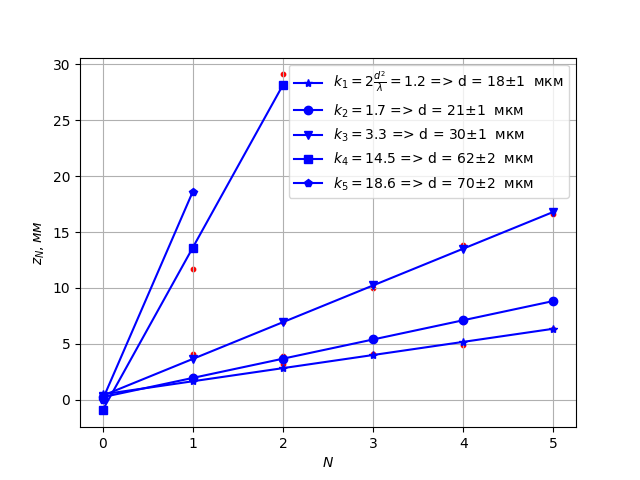
\includegraphics[scale=0.9]{z(N).png}}
			\caption{График зависимости $z_N(N)$ и расчет периода для каждой сетки}
		\end{figure}
		
		
		\textbf{Обсуждение результатов и выводы: }\\
		
		\begin{longtable}{|c|c|c|c|}
			\hline
			
			№ & Саморепродукция, d мкм & Линза, d мкм & Дифракция, d мкм \\ \hline
			1 & 18$\pm 1$ & 42$\pm 20$& 20,7$\pm 0,3$\\ \hline
			2 & 21$\pm 1$ & 63$\pm 20$ & 29,9$\pm 0,4$\\ \hline
			3 & 18$\pm 1$ & 84$\pm 20$ & 60$\pm 1$\\ \hline
			4 & 18$\pm 2$ & 126$\pm 20$ & 120$\pm 2$\\ \hline
			5 & 18$\pm 2$ & 147$\pm 20$ & 157$\pm 2$\\ \hline
			\caption{Сводная таблица полученных результатов для периодов решеток тремя различными способами}
		\end{longtable}
		
		В данной работе мы наблюдали эффект саморепродукции, определили с помощью данного эффекта периоды различных решеток. Сравнили полученные результаты с результатами других опытов для определения периода решетки: методом линзы и дифракции.
		
		По полученным результатам стоит отметить, что более точный результат получился методом дифракции. Метод линзы плохо показал себя на сетках с малым периодом, а метод саморепродукции наоборот на сетках с наибольшим периодом. Эти результаты объясняются большой погрешностью измерения малых расстояний в первом случае и больших расстояний во втором.
		
		
		
	\end{enumerate}
	
	
	
	
	
	
	
	
	
	
	
	
	
	
	
	
	
	
	
	
	
	
	
	
	
	
	
	\end{document}